\subsubsection{UML Class Diagram}
\label{sec:backend-class-diagram}

The UML class diagram displayed in Figure \ref{fig:expense-class-diagram} provides a static, focused view of the main classes involved in the core Expense use case. This diagram is the concrete blueprint that visually represents how the abstract concepts of Clean Architecture are translated into code for a primary functional area. 

Building on this blueprint, the diagram illustrates the relationships between the \texttt{Expense- Controller}, the \texttt{IExpenseService}, and the \texttt{IExpenseRepository}, as well as their implementations. It also demonstrates the application of the main architectural principles, patterns, and design approaches explained in Section \ref{sec:principles-and-patterns}. 

\begin{figure}[H]
    \centering
    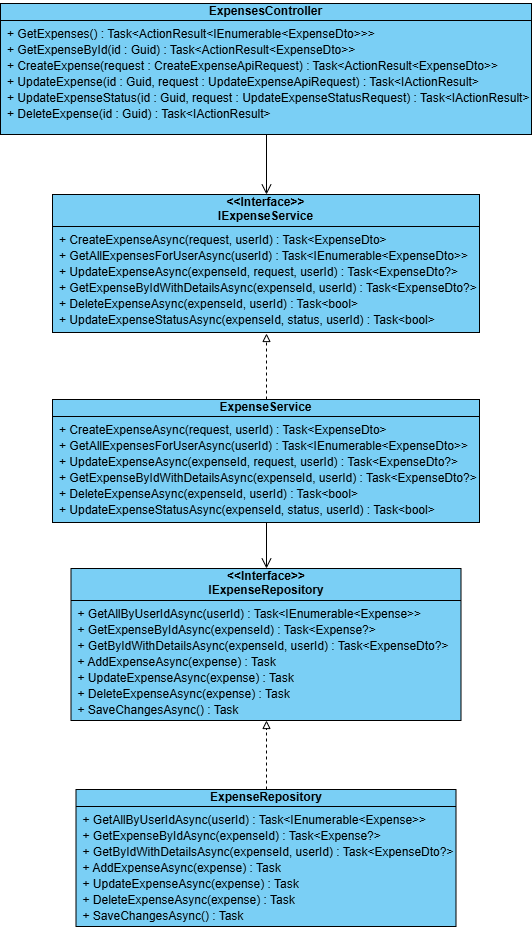
\includegraphics[width=0.7\textwidth]{Images/backend/ExpenseClassDiagram.png}
    \caption[Backend UML class diagram focused on Expense functionality]
    {Backend UML class diagram focused on Expense functionality. [Own creation]}
    \label{fig:expense-class-diagram}
\end{figure} 

A detailed UML class diagram covering all classes within the backend's logical layers has also been created to ensure a complete system model. Due to its size and level of detail, it is provided in Appendix \ref{appendix:uml-class-diagram}. Given the diagram's complexity, the Domain and DTO classes are omitted, although they are implicitly included within each class's operations. For a more detailed domain diagram, please refer to Figure \ref{fig:database-schema-diagram}.
